\documentclass[dvisvgm,border=2pt]{standalone}
% Shared by every figure. Two colours only: black becomes the text colour of
% whatever theme the app is in, and `accent` becomes the brand — see
% scripts/build-figures.mjs. Everything else is done with opacity.
\usepackage{amsmath}
\usepackage{amssymb}
\usepackage{tikz}
\usepackage{pgfplots}
\pgfplotsset{compat=1.18}
\usetikzlibrary{arrows.meta,positioning,calc,backgrounds,fit,patterns.meta}
\definecolor{accent}{RGB}{255,0,255}
\pgfplotsset{
  every axis/.append style={
    axis lines=left,
    axis line style={draw opacity=0.35},
    tick style={draw opacity=0.35},
    tick label style={font=\scriptsize,opacity=0.7},
    label style={font=\scriptsize,opacity=0.7},
    legend style={draw=none,fill=none,font=\scriptsize},
    every axis plot/.append style={line width=0.7pt},
  },
}
\tikzset{
  every picture/.style={font=\scriptsize},
  faint/.style={opacity=0.3},
  quiet/.style={opacity=0.55},
  box/.style={draw,opacity=0.35,rounded corners=2pt,inner sep=4pt},
  hot/.style={accent},
}

\begin{document}
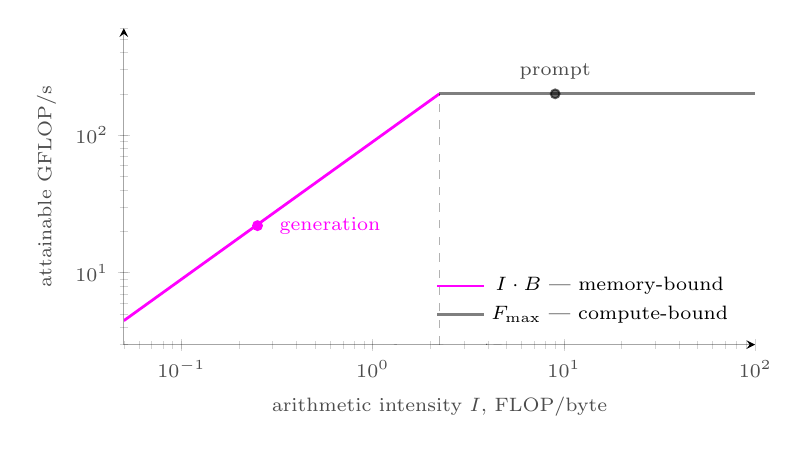
\begin{tikzpicture}
  \begin{loglogaxis}[width=9.6cm,height=5.6cm,
      xlabel={arithmetic intensity $I$, FLOP/byte},
      ylabel={attainable GFLOP/s},
      xmin=0.05,xmax=100,ymin=3,ymax=600,
      legend style={at={(0.98,0.03)},anchor=south east}]
    % memory roof: I * B, with B = 89.6 GB/s; compute roof 200 GFLOP/s
    \addplot[accent,line width=1pt,domain=0.05:2.232,samples=2]{89.6*x};
    \addlegendentry{$I\cdot B$ — memory-bound}
    \addplot[opacity=0.5,line width=1pt,domain=2.232:100,samples=2]{200};
    \addlegendentry{$F_{\max}$ — compute-bound}
    \draw[opacity=0.3,dashed] (axis cs:2.232,3) -- (axis cs:2.232,200);
    \node[opacity=0.6,anchor=north,font=\scriptsize] at (axis cs:2.232,3.6) {ridge $F_{\max}/B$};
    \addplot[only marks,mark=*,accent,mark options={scale=0.8}] coordinates {(0.25,22)};
    \node[accent,anchor=west,font=\scriptsize] at (axis cs:0.29,22) {generation};
    \addplot[only marks,mark=*,opacity=0.6,mark options={scale=0.8}] coordinates {(9,200)};
    \node[opacity=0.7,anchor=south,font=\scriptsize] at (axis cs:9,215) {prompt};
  \end{loglogaxis}
\end{tikzpicture}
\end{document}
